\section{Arhitektura FPGA} \label{a}
FPGA so vezja za implementacijo specializirane logike.

Narejena so iz množice spominskih in kombinatoričnih celic.
Kombinatorične celice so mali kosi spomina, s katerimi definiramo pravilnostno tabelo naše funkcije.
Spominske celice so navadni DFF.
Pomembna stvar so povezave med celicami, ki so konfigurabilne. To pomeni, da mi določimo pravilnostne tabele in povezave med njimi. 

Obstajajo tudi prenosne verige, reset in clk linije in vgrajeni spomin, množilniki CPU ect.

Ima možnost povratne vezave, tako da lahko gledamo kot max preprost turing machine???, na sploh lohk iz teh blokov zelo lahko delamo vezja po kopitu register,logika,register...ect


\subsection{FPGA Celice}
FPGA Celica zgleda pribljižno takole:

\begin{figure}
	\centering
	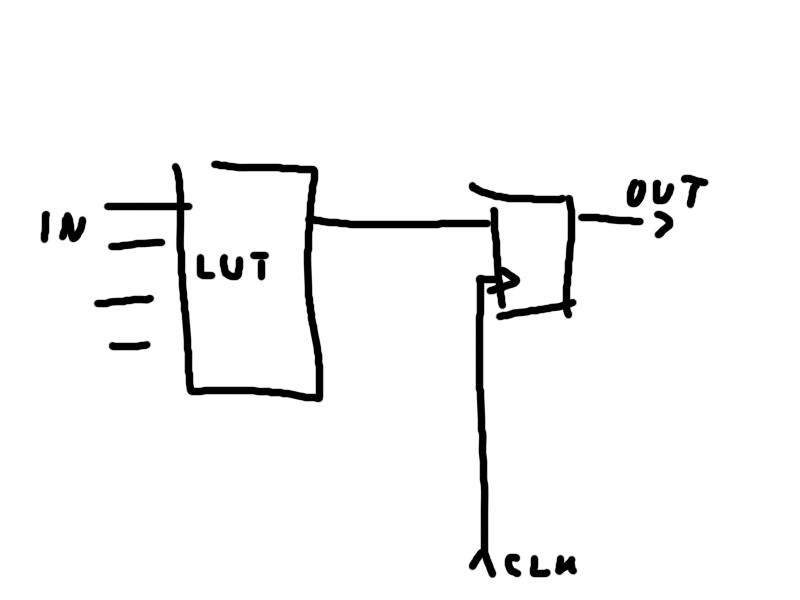
\includegraphics[width=0.7\linewidth]{slike/cell}
	\caption{}
	\label{fig:cell}
\end{figure}

\subsubsection{LUT}

Lut je mehn košček spomina. Notr ma par bitou, direk implemenira tabelo

\subsubsection{FF}

FF je preprost FF, ima puno option bitov ect

\subsection{FPGA povezave}

Povezave so večino površine, grejo med celicami, so programibilne, torej imajo puno tranzistorjev, torej zakasnitve...

\begin{figure}
	\centering
	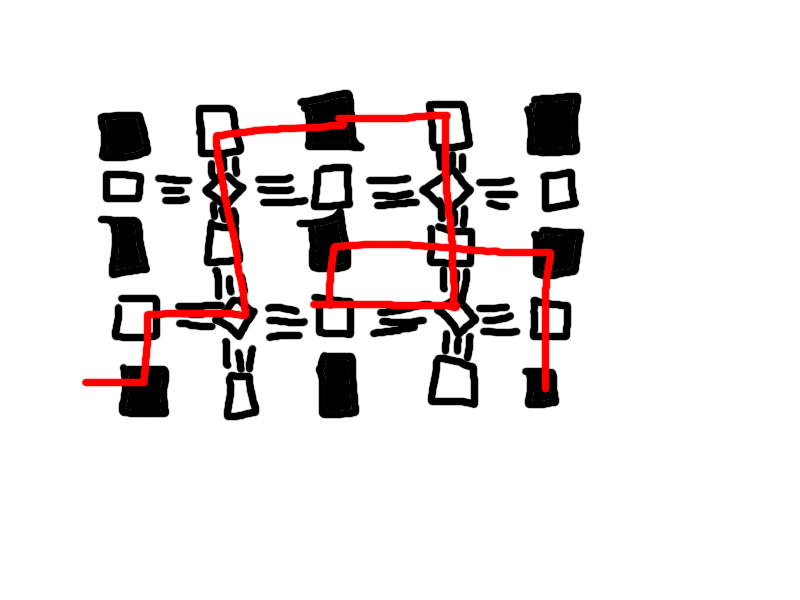
\includegraphics[width=0.7\linewidth]{slike/routing}
	\caption{}
	\label{fig:cell}
\end{figure}

\section{Verilog} \label{a}
Jezik za opis procesov, uporablja se za programiranje FPGA

\section{Implementacija} \label{a}
\subsection{4-Phase dual rail} \label{b}
Za impelementacijo tega protokola potrebujemo posplošene C elemente, Logika je narejena iz spominskih celic, data/ null waves ect

\subsection{2-Phase dual rail} \label{b}
Podobno, kot pri 4 Phase ampak uporabljamo robove, potrebujemo več tranzistorjev za logiko, saj potrebujemo povratno informacijo, od izhodov


\subsection{Implementacija cellic} \label{a}
\subsubsection{Primitivi} \label{b}
Imamo 5 Primitivov, iz katerih sestavimo ostalo funkcionalnost vezja:

C muller C, razne implementacije, rezultati
P za TP
C splošno, drevesna struktura
ect


\subsubsection{Funkcionalne celice} \label{b}
injektorji pričnejo delovanje cikla
cmpl det preveri če je stanje validno
adder sestevalnik
mem reg spominska celica


\subsubsection{Vezja} \label{b}
FIB fibbonacci counter, 1,2,3,5,8,13 toy example predstavi inicalizacijo

GCD, ciklična komputacija, preprostejša inicializacija

RISCV čim bolj preprost processor, proof of concept